\documentclass{beamer}
\usepackage[utf8]{inputenc} % 한글 입력을 위해
\usepackage{kotex}          % 한글 사용 패키지
\usepackage{graphicx}       % 이미지 포함을 위해

% 테마 설정 (다양한 테마가 있습니다: Madrid, Boadilla, Warsaw 등)
\usetheme{Madrid}
\usecolortheme{default}

\title{강원도 강수량 시계열 분석}
\subtitle{ARIMA 모델을 이용한 예측}
\author{이태녕}
\date{\today}

\begin{document}

% 제목 슬라이드
\begin{frame}
    \titlepage
\end{frame}

\frametitle{강원도 지역별 데이터}

\begin{frame}{데이터 시각화: 강원도 월별 강수량}
    \begin{figure}
        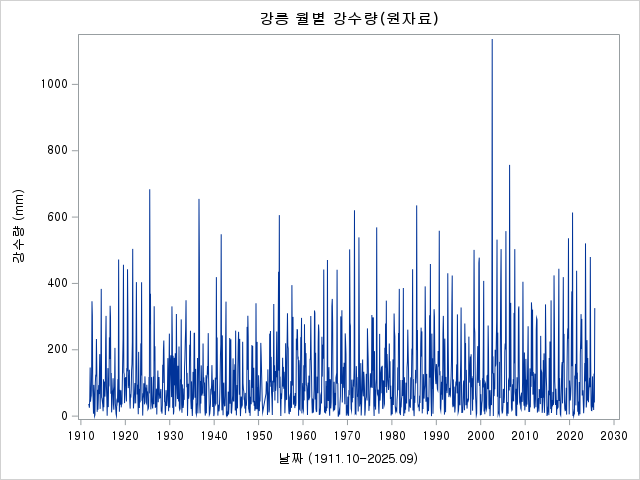
\includegraphics[width=0.9\textwidth]{alldata.png}
        \caption{1993-2023년 월별 강수량 시계열 그래프}
    \end{figure}
\end{frame}


\begin{frame}{모델 식별: 기본 ACF/PACF 그래프}
    \begin{figure}
        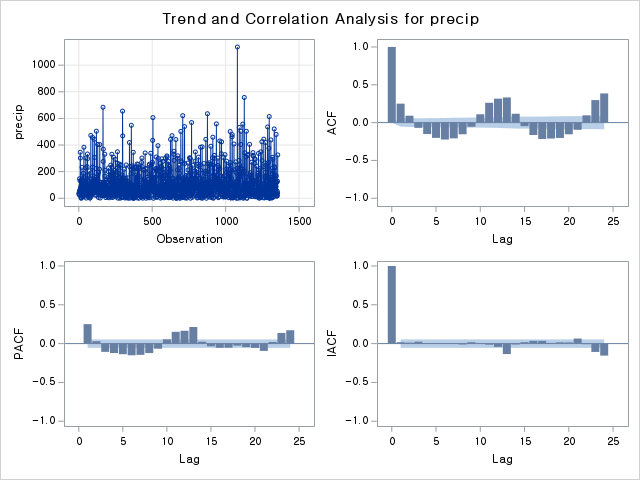
\includegraphics[width=0.9\textwidth]{alldata_acf.png}
        \caption{ACF/PACF 그래프}
    \end{figure}
\end{frame}


\begin{frame}{모델 식별: 1차 차분 ACF/PACF 그래프}
    \begin{figure}
        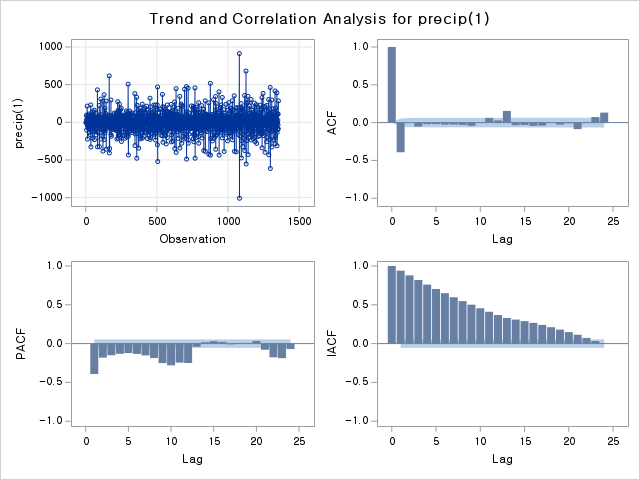
\includegraphics[width=0.9\textwidth]{alldata_acf_1.png}
        \caption{ACF/PACF 그래프}
    \end{figure}
\end{frame}

\begin{frame}{모델 식별: SAS Macro로 최소 AIC 값 가지는 모수 찾기}
\begin{table}[h!]
\centering
\caption{모수별 AIC (하위 5개)}
\label{tab:model_comparison}
\begin{tabular}{cccccc}
\hline
\textbf{OBS} & \textbf{p} & \textbf{q} & \textbf{sp} & \textbf{sq} & \textbf{AIC} \\ \hline
1            & 0          & 1          & 1           & 2           & 16053.36     \\
2            & 0          & 1          & 0           & 2           & 16054.00     \\
3            & 0          & 2          & 1           & 1           & 16054.97     \\
4            & 0          & 2          & 0           & 2           & 16055.42     \\
5            & 1          & 1          & 1           & 1           & 16055.96     \\ \hline
\end{tabular}
\end{table}
\end{frame}

\begin{frame}{ARIMA(0,1,1)(1,1,2)}
    \begin{figure}
        \centering
        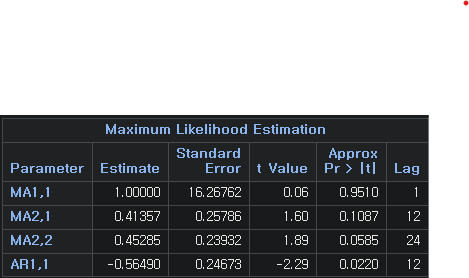
\includegraphics[width=0.9\textwidth]{model1.png}
        \caption{noint option, 단위근 발견}
    \end{figure}
\end{frame}

\begin{frame}{ARIMA(0,1,1)(0,1,2)}
    \begin{figure}
        \centering
        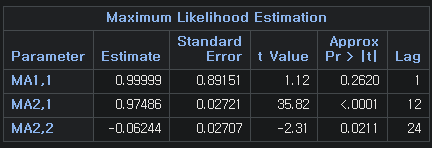
\includegraphics[width=0.9\textwidth]{model2.png}
    \end{figure}
\end{frame}

\begin{frame}{ARIMA(0,1,1)(0,1,2) ACF/PACF}
    \begin{figure}
        \centering
        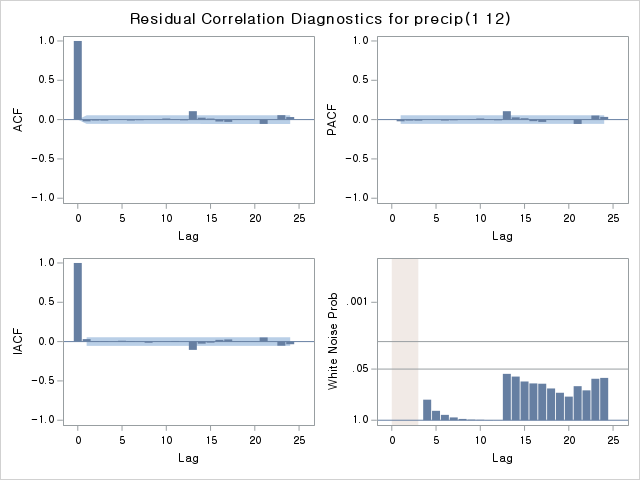
\includegraphics[width=0.9\textwidth]{model2_acf.png}
    \end{figure}
\end{frame}

\begin{frame}{ARIMA(0,1,1)(0,1,2) Forecast}
    \begin{figure}
        \centering
        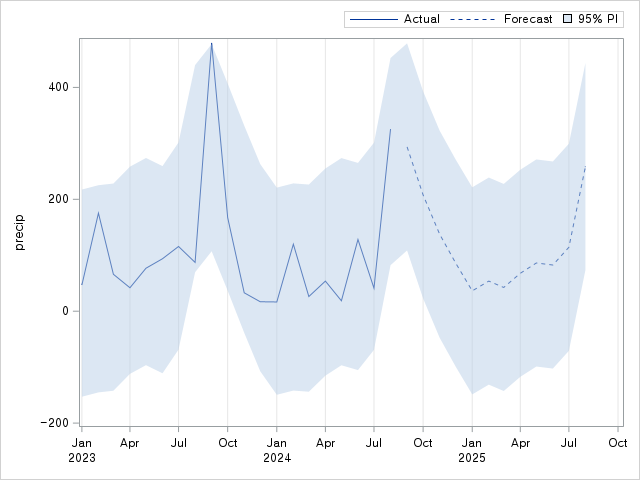
\includegraphics[width=0.9\textwidth]{modelresult.png}
    \end{figure}
\end{frame}


% \begin{frame}{SARIMA 모델 추정 결과}
%     % \begin{table}
%     %     \centering
%     %     \caption{SARIMA(0,0,1)(0,1,1)\(_ {12}\) 모수 추정치}
%     %     \begin{tabular}{|l|c|c|c|}
%     %         \hline
%     %         \textbf{Parameter} & \textbf{Estimate} & \textbf{Std Error} & \textbf{t Value} \\
%     %         \hline
%     %         MA1,1 (비계절성) & 0.35 & 0.05 & 7.00 \\
%     %         MA2,1 (계절성) & -0.85 & 0.03 & -28.33 \\
%     %         \hline
%     %     \end{tabular}
%     %     \medskip
%     %     \begin{itemize}
%     %         \item AIC: 4500.5
%     %         \item SBC: 4510.2
%     %     \end{itemize}
%     % \end{table}
% \end{frame}

% \begin{frame}{미래 강수량 예측 (24개월)}
%     % \begin{figure}
%     %     \includegraphics[width=0.9\textwidth]{C:/your_path/sas_outputs/arima_plotsForecast.png}
%     %     \caption{SARIMA 모델 기반 예측 (점선: 예측값, 음영: 95\% 신뢰구간)}
%     % \end{figure}
% \end{frame}

\end{document}